\documentclass[a4paper,10.5pt]{article}
%\documentclass[10pt]{article}
\usepackage[T1]{fontenc}
\usepackage[utf8]{inputenc}
\usepackage{lmodern}
\usepackage[english]{babel}

\usepackage{amsmath}
\usepackage{amssymb}
\usepackage{tikz}
\usepackage{multicol}
\usepackage{enumitem}

\usepackage[top=.25cm, bottom=.25cm, left=.25cm, right=.25cm]{geometry}

\newcommand{\com}[1]{#1}  
\renewcommand{\com}[1]{}
\newcommand{\ud}{\mathrm{d}}
\newcommand{\N}{\mathbb{N}}
\newcommand{\R}{\mathbb{R}}
\newcommand\independent{\protect\mathpalette{\protect\independenT}{\perp}}
\def\independenT#1#2{\mathrel{\rlap{$#1#2$}\mkern2mu{#1#2}}}


\setlength{\parindent}{0pt}

\begin{document}
	\begin{multicols}{4}
		\setlength{\columnseprule}{1pt}
		\textbf{Intro}
		
		\textbf{Mean} : $\overline{x} = \frac{1}{n} \sum_{i=1}^{n} x_i$
		
		\textbf{Quantile} : $q_p = x_{(1+(n-1)p)}$
		
		\textbf{Range} : $Max-min = q_1 - q_0$
		
		\textbf{IQR} : $q_{0.75} - q_{0.25}$
		
		\textbf{Outliers} : $< q_{0.25} - 1.5 IQR$
		
		\textbf{boxplot} :
		
		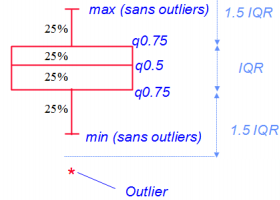
\includegraphics[width=4.8cm]{img/boxplot.PNG}
		
		\textbf{Sample Variance} : $s^2 = \frac{1}{n-1}\sum_i (x_i - \overline{x})^2$
		
		\textbf{Sample Standard Deviation} (SD) : $s = \sqrt{s^2}$
		
		\textbf{Coefficient of Variation} : $cv = \frac{s}{\overline{x}}$
		
		\textbf{Probabilities}
		
		\textbf{Simple event} : event with only 1 outcome.
		
		\textbf{Sample space} : discrete (countable) vs continuous.
		
		certain event (S) vs impossible event ($\emptyset$).
		
		$P(S) = 1$
		
		$0 \leq P(A) \leq 1\ \forall A$
		
		$P(A) = \frac{\# favorable}{\# possible}$
		
		$P(A) = \lim_{N \to \infty} \frac{\#A\ observed }{\#observed}$
		
		$P(\overline{A}) = 1-P(A)$
		
		$P(A \cup B) = P(A) + P(B) - P(A\cap B)$
		
		$P(A|B) = \frac{P(A\cap B)}{P(B)}$
		
		Events mutually \textbf{independent} if : $P(\cap_{i} A_i) = \prod_i P(A_i)$
		
		\textbf{permutation} (order) vs \textbf{combination}
		
		$A_n^r = \frac{n!}{(n-r)!}$ (r (from n) ordered distinct objects)
		
		$C_n^r = (_r^n) = \frac{A_n^r}{r!}$ : (r (from n) unordered distinct objects)
		
		
		discrete (countable) vs Continuous (noted d) vs c))
		
		d) \textbf{probability mass function} (\textbf{pmf}) : $p(x) = P(X=x)\ \forall x\in X$
		
		d) $p(x)>0\ if\ x\in R,\ p(x) = 0\ if\ x\notin R,\ \sum p(x_i) = 1$
		
		c) $P(X=x)=0\ \forall x\in R$
		
		c) \textbf{probability density function} (\textbf{pdf}) : $ f(x)\ tq\ P(X\in I) = \int_I f(x) dx$
		
		c) $\int_{-\infty}^{\infty} f(x) dx = 1$
		
		\textbf{cumulative distribution function} (\textbf{cdf}) : $F(x) = P(X\leq x)$
		
		d) $F(x) = \sum_{x_i\leq x} p(x_i)$
		
		c) $F(x) = \int_{-\infty}^{x} f(t) dt$
		
		$x<y \Rightarrow F(x) \leq F(y)$
		
		$F(-\infty ) = 0\ and\ F(+\infty )=1$
		
		$F(x^+) = F(x)$
		
		$P(a<X\leq b) = F(b) - F(a)$
		
		c) $f(x) = F'(x)$
		
		$\mathbb{E}(X) \equiv \mu_X$
		
		d) $\mathbb{E}(h(X)) = \sum h(x)\ p(x)$
		
		c) $\mathbb{E}(h(X)) = \int_{-\infty}^{\infty}h(x)\ f(x)dx$
		
		$k^{th}$ \textbf{moment of X} : $\mathbb{E}(X^k)$
		
		$\mathbb{E}(\sum X_i) = \sum \mathbb{E}(X_i)$
		
		\textbf{Variance} : $Var(X) \equiv \mathbb{V}(X) \equiv \sigma_X^2 = \mathbb{E}(X-\mu_X)^2 = \mathbb{E}(X^2) - (\mathbb{E}(X))^2$
		
		$\mathbb{V}(a+bX) = b^2 \mathbb{V}(X)$
		
		\textbf{standard deviation} : $\sigma_X = \sqrt{\sigma_X^2}$
		
		Markov inequality : $P(|X| \geq a) \leq \frac{\mathbb{E}|X|}{a},\ \forall a>0$
		
		Chebychev inequality : $P(|X-\mu_X| \geq k*\sigma_X) \leq \frac{1}{k^2},\ \forall k>0$
		
		\textbf{Quantile} of order p of X : $P(X<q_p) \leq p \leq P(X\leq q_p)$
		
		c) $q_p = F^{-1}(p)$
		
		\textbf{moment generating function} (\textbf{mgf}) : $m_X(t) = \mathbb{E}(e^{tX})$ (if it exists $\forall\  |t|<\epsilon$)
		
		$\left.\dfrac{\ud^k m_x(t)}{\ud t^k}\right|_{t=0} = \mathbb{E}(X^k)$
		
		$m_X(t) = m_Y(t),\ \forall |t|<\epsilon \Rightarrow X =_d Y$
		
		$m_{a+bX}(t) = e^{at}m_X(bt)$
		
		\textbf{Discrete distributions}
		
		\textbf{uniform} : $P(X = x_i) = \frac{1}{n}$
		
		$\mu_X = \frac{\sum x_i}{n}\ \&\ \sigma_X^2 = \frac{\sum x_i^2}{n}-\mu_X^2$
		
		\textbf{Bernouilli} $\sim Be(p)$ : success or failure.
		
		$P(X=1) = p\ \&\ P(X=0) = q = 1-p$
		
		$\mu_X = p\ \&\ \sigma_X^2 = pq$
		
		\textbf{Binomial} $\sim Bi(n,p)$ : \#success of n Be(p).
		
		$P(X=x) = C_n^x p^x q^{(n-x)}$
		
		$m_x(t) = (pe^t+q)^n$
		
		$\mu_X = np\ \&\ \sigma_X^2 = npq$
		
		\textbf{Geometric} $\sim Ge(p)$ : \#Be(p) until success.
		
		$P(X=x) = q^{x-1}p (x=1,2,...)$
		
		$m_x(t) = \frac{pe^t}{1-qe^t}$ ($t<-\ln(q)$)
		
		$\mu_X = \frac{1}{p}\ \&\ \sigma_X^2 = \frac{q}{p^2}$
		
		\textbf{Poisson} $\sim Po(\lambda)$ : if $\lambda$ event/year (rate), \#event this year. $Bi(n,\lambda/n) \overset{n=\infty}\longrightarrow Po(\lambda)$. (each infinitely small moment is a Bernouilli trial).
		
		$P(X=x) = e^{-\lambda}\frac{\lambda^x}{x!}$
		
		$m_X(t) = e^{\lambda(e^t-1)}$
		
		$\mu_X = \sigma_X^2 = \lambda$
		
		\textbf{Negative binomial} $\sim NB(r,p)$ : \#Be(p) until r success.
		
		\textbf{Hypergeometric} $\sim Hyp(n,r,N)$ : \#ones when taking n numbers from r ones and N-r zeros.
		
		\textbf{Continuous distributions}
		
		\textbf{Uniform} $\sim U(a,b)$ : $f(x) = \frac{1}{b-a}\ if\ x\in [a,b]$
		
		$F(x) = \frac{x-a}{b-a}\ if\ x\in [a,b]$, 0 or 1 else.
		
		$m_X(t) = \frac{e^{tb}-e^{ta}}{t(b-a)}$
		
		$\mu_X = \frac{a+b}{2}\ \&\ \sigma_X^2 = \frac{(b-a)^2}{12}$
		
		\textbf{Normal} $\sim \mathcal{N}(\mu,\sigma^2)$ : $f(x) = \frac{1}{\sigma \sqrt{2\pi}}e^{-\frac{1}{2}}(\frac{x-\mu}{\sigma})^2$
		
		$F(x) = see\ tables$
		
		$m_X(t) = e^{\mu t + \frac{t^2\sigma^2}{2}}$
		
		$\mu_X = \mu\ \&\ \sigma_X^2 = \sigma^2$
		
		$f"(\mu\pm\sigma) = 0$ 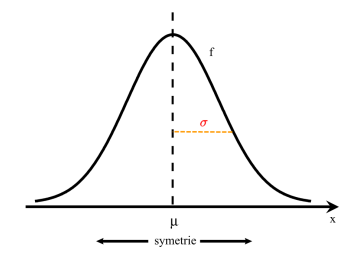
\includegraphics[width=1 cm]{img/normal.PNG}
		
		$P(Z\geq z_\alpha) = \alpha\ (Z \sim \mathcal{N}(0,1)) \Rightarrow z_\alpha = q_{1-\alpha}$
		
		$X \sim \mathcal{N}(\mu, \sigma^2) \Rightarrow a+bX \sim \mathcal{N}(a+b\mu,b^2\sigma^2) \Rightarrow \frac{X-\mu}{\sigma} \sim \mathcal{N}(0,1)$
		
		$q_{1-\alpha} = \sigma z_\alpha + \mu$ (for $\mathcal{N}(\mu,\sigma^2)$)
		
		\textbf{Gamma} $\sim Gamma(\alpha,\beta)$ : $f(x) = \frac{x^{\alpha-1}e^{-x/\beta}}{\beta^\alpha \Gamma(\alpha)}$ for $x \geq 0$
		
		$\alpha,\beta > 0\ \&\ \Gamma(\alpha) = \int_0^\infty t^{\alpha-1}e^{-t} dt$
		
		$\Gamma(\alpha+1) = \alpha \Gamma(\alpha)$
		
		$m_X(t) = (1-\beta t)^{-\alpha}\ (t<1/\beta)$
		
		$\mu_X = \alpha\beta\ \&\ \sigma_X^2 = \alpha\beta^2$
		
		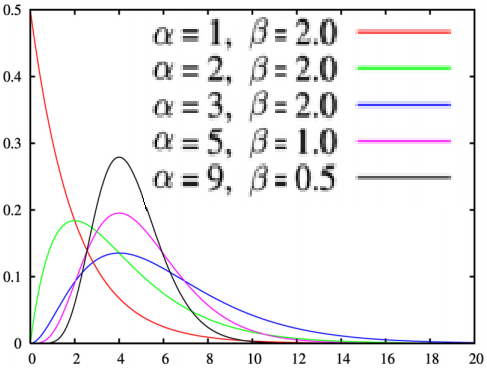
\includegraphics[width=3 cm]{img/gamma.PNG}
		
		\textbf{Exponential} $\sim Expo(\beta) \equiv Gamma(1,\beta)$ : time between Poisson events (rate = 1/$\beta$).
		
		$P(X\leq t+x | X>t) = P(X\leq x)$
		
		\textbf{Chi-square} with n degrees of freedom $\sim \chi_n^2 \equiv Gamma(n/2,2)$
		
		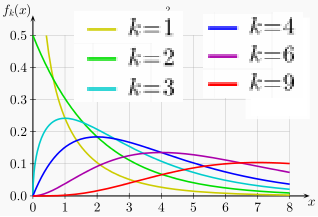
\includegraphics[width=4cm]{img/chi.PNG}
		
		\textbf{Multivariate probability distributions}
		
		\textbf{random vector} (discrete (countable \#elements) vs continuous)
		
		distributions : \textbf{joint} (j)), \textbf{marginal} (m)), \textbf{conditional} (cd)).
		
		j d) $p(x,y) = P(X=y, Y=y)$
		
		j c) $P((X,Y)\in A) = \iint_A f(x,y) dx dy$
		
		j) $F(x,y) = P(X\leq x,Y\leq y)$
		
		j) $f(s,t) = \frac{\partial^2F}{\partial x\partial y}(s,t)$
		
		m d) $p_X(x) = P(X=x) = \sum_y P(X=x, Y=y)$
		
		m c) $f_X(x) = \int_{-\infty}^\infty f(x,y)dy$
		
		m) $F_X(x) = P(X \leq x) = F(x,\infty)$
		
		d) $p(y|x) = \frac{p(x,y)}{p_X(x)}$ (p$\to$f for c))
		
		r.v. independent if 
		
		$P(X\in A, Y\in B) = P(X\in A) P(Y\in B) \ \forall A, B$
		
		$\Leftrightarrow F(x,y) = F_X(x)F_Y(y)$
		
		$\Leftrightarrow f(x,y) = f_X(x)f_Y(y)$
		
		$\Leftrightarrow f(y|x) = F_Y(y)$
		
		$\Leftrightarrow m_{X+Y}(t) = m_X(t)m_Y(t)$
		
		cd) $\mathbb{E}(g(Y)|X=x) = \int g(y) f(y|x) dy$
		
		$\mu_Y(x) = \mathbb{E}(Y|X=x)$
		
		$\sigma_Y^2(x) \equiv \mathbb{V}ar(Y|X=x) = \mathbb{E}(Y^2|X = x) - \mu_Y^2(x)$
		
		c) $\mathbb{E}(g(X,Y)) = \iint g(x,y)f(x,y)dxdy$
		
		$\mathbb{E}(X+Y) = E(X) + E(Y)$
		
		$\mathbb{E}(XY) = \mathbb{E}(X)\mathbb{E}(Y) if X\independent Y$
		
		$\mathbb{V}ar(X+Y) = \mathbb{V}ar(X) + \mathbb{V}ar(Y) + 2(\mathbb{E}(XY) - \mathbb{E}(X)\mathbb{E}(Y))$
		
		$m_{X,Y}(s,t) \equiv m(s,t) = \mathbb{E}(e^{sX+tY})$
		
		$\dfrac{\partial^{k+n} m}{\partial s^k \partial t^n}(0,0) = \mathbb{E}(X^kY^n)$
		
		$m(s,0) = m_X(s)$
		
		$\sigma_{XY} \equiv \mathbb{C}ov(X,Y) = \mathbb{E}(XY)-\mathbb{E}(X)\mathbb{E}(Y)$
		
		$\mathbb{C}ov(X,a+bX) = b\mathbb{V}ar(X)$
		
		$\mathbb{C}ov(X,Y)>0$ if X and Y have tendancy to vary in the same direction.
		
		$X\independent Y \Rightarrow \mathbb{C}ov(X,Y) = 0$
		
		$\mathbb{C}ov(aX + bY,Z) = a\mathbb{C}ov(X,Z) + b\mathbb{C}ov(Y,Z)$
		
		$\mathbb{V}\left(\sum a_iX_i\right) = \sum a_i^2 \mathbb{V}(X_i) + 2 \sum a_ia_j\mathbb{C}ov(X_i,X_j)$
		
		$\rho_{XY} \equiv \rho(X,Y) = \frac{\sigma_{XY}}{\sigma_X\sigma_Y}$
		
		$|\rho_{XY}|\leq 1$
		
		$\rho_{XY} = \pm 1 \Leftrightarrow Y = a + bX$
		
		$\mathbb{E}(Y) - b\mathbb{E}(X) + \frac{\rho_{XY}}{\sigma_X^2}X$ is the best linear approximation of Y.
		
		\textbf{multivariate distributions}
		
		\textbf{Multinomial distribution} : multi Bi(n,p).
		
		$P(X_1 = x_1, ..., X_d = x_d) = \frac{n!}{\prod x_i !}\prod p_i^{x_i}$ for $\sum x_i = n$
		
		$X_i \sim Bi(n,p_i)$ and $\mathbb{C}ov(X_i,X_j) = -np_ip_j$
		
		\textbf{Bivariate Normal} : multi $\mathcal{N}(\mu,\sigma^2)$.
		
		$f(x_1,x_2) = \frac{1}{2\pi\sigma_1\sigma_2\sqrt{1-\rho^2}}e^{-\frac{Q(x_1,x_2)}{2(1-\rho^2)}}$
		
		$Q(x_1,x_2) = \sum \left(\frac{x_i-\mu_i}{\sigma_i}\right)^2 - 2\rho\prod \left(\frac{x_i-\mu_i}{\sigma_i}\right)$
		
		$\mu_i = \mu_{X_i}, \sigma_i^2 = \sigma_{X_i}^2$ and $\rho = \rho_{X_1X_2}$
		
		$X_i \sim N(\mu_i,\sigma_i^2)$ \& $X_1 \independent X_2 \Rightarrow (X_1,X_2) \sim N_2$ with $\rho=0$
		
		$(X_1,X_2)\sim N_2 \Rightarrow \left(X_1 \independent X_2 \Leftrightarrow \rho = 0\right)$
		
		$(X_1,X_2) \sim N_2 \Leftrightarrow aX_1+bX_2 \sim N$
		
		\textbf{Functions of r.v.}
		
		c) Y=g(X), g differentiable, strictly monotonic : $f_Y(y) = \left.\frac{f_X(x)}{|g'(x)|}\right|_{x=g^{-1}(y)}$
		
		\textbf{Lognormal} $\sim LN(\mu,\sigma^2)$ : $Y\sim N(\mu,\sigma^2) \Rightarrow X=e^Y \sim LN(\mu,\sigma^2)$ 
		
		$f(x) = \frac{1}{x\sqrt{2\pi\sigma^2}}e^{-\frac{1}{2}\left(\frac{\ln x - \mu}{\sigma}\right)^2}$
		
		$\mu_X = e^{\mu+\sigma^2/2}\ \&\ \sigma_X^2 = (e^{\sigma^2}-1)e^{2\mu+\sigma^2}$
		
		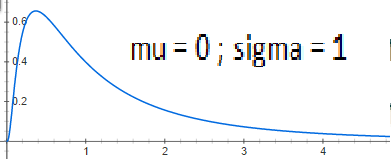
\includegraphics[width=4cm]{img/ln.png}
		
		g not monotonic : $f_Y(y) = \sum_{x\in g^{-1}(y)} \frac{f_X(x)}{|g'(x)|}$
		
		$X\sim N(0,1) \Rightarrow Y=X^2\sim \chi_1^2$
		
		$X = \left(^{X_1}_{X_2}\right)\  _{\leftarrow_{g^{-1}}}^{\to^g} \left(^{Y_1}_{Y_2}\right) = Y$
		
		$\Rightarrow f_Y(y) = \left.\frac{f_X(x)}{|Jac_g(x)|}\right|_{x=g^{-1}(y)}$
		
		$|Jac_g(x)| = \left|\frac{\partial g_1}{\partial x_1}\frac{\partial g_2}{\partial x_2}-\frac{\partial g_1}{\partial x_2}\frac{\partial g_2}{\partial x_1}\right|(x)$
		
		$Z=g(X,Y) \Rightarrow F_Z(z) = \iint_{(g(x,y) \leq z)}f(x,y)dxdy$
		
		$f_{XY}(z) = \int_{-\infty}^\infty \frac{1}{|y|}f(z/y,y)dy$
		
		$(X\independent Y) \sim N(0,1) \Rightarrow Z = Y/X \sim$ \textbf{standard Cauchy density} :
		
		$f_Z(z) = \frac{1}{\pi(z^2+1)}$
		
		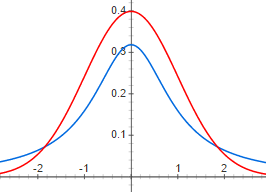
\includegraphics[width=2cm]{img/Cauchy.PNG} (cauchy(b) vs N(0,1) (r))
		
		Using $m_{X+Y}=m_Xm_Y$ :
		
		$Y = \sum^n ((\independent X_i) \sim Gamma(\alpha_i,\beta)) \sim Gamma(\sum^n\alpha_i,\beta)$
		
		$Y = \sum^n ((\independent X_i) \sim Expo(\beta)) \sim Gamma(n,\beta)$
		
		$Y = \sum^n ((\independent X_i) \sim \chi_1^2) \sim \chi_n^2$
		
		$Y = \sum^n ((\independent X_i) \sim N(\mu_i,\sigma_i^2)) \sim N(\sum^n \mu_i, \sum^n \sigma_i^2)$
		
		\textbf{t-distribution} with n degrees of freedom $\sim t_n$ : $X\sim N(0,1) \independent Y\sim\chi_n^2 : Z = \frac{X}{\sqrt{Y/n}} \sim t_n$
		
		$f(z) = \frac{\Gamma(\frac{n+1}{2})}{\sqrt{n\pi}\Gamma(n/2)}\left(1+\frac{z^2}{n}\right)^{-\frac{n+1}{2}}$
		
		$t_n \overset{n\to\infty}\longrightarrow N(0,1)$ (n>30 is enough)
		
		$t_1$ = standard Cauchy.
		
		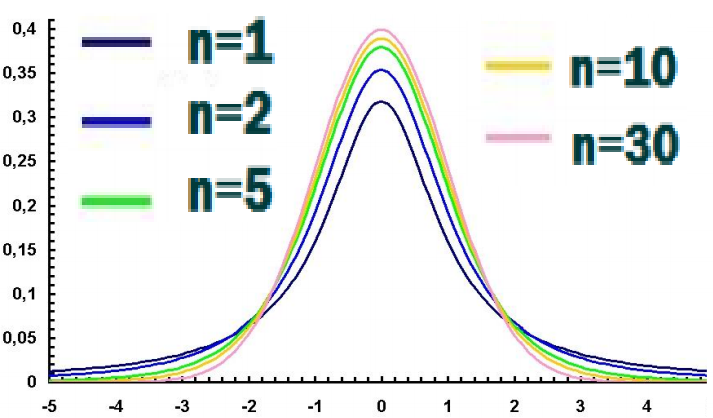
\includegraphics[width=4cm]{img/t.PNG}
		
		\textbf{F-distribution} with $n_1$ and $n_2$ degrees of freedom $\sim \mathcal{F}_{n_1,n_2}$ : $(X_1\independent X_2) \sim \chi_{n_i}^2 \Rightarrow Z = \frac{X_1/n_1}{X_2/n_2} \sim \mathcal{F}_{n_1,n_2}$
		
		$f(z) = \frac{\Gamma((n_1+n_2)/2)}{\Gamma(n_1/2)\Gamma(n_2/2)} (n_1/n_2)^{n_1/2}$
		
		$\frac{z^{n_1/2-1}}{(1+n_1z/n_2)^{(n_1+n_2)/2}}$
		
		$F\sim \mathcal{F}_{n_1,n_2} \Rightarrow 1/F \sim \mathcal{F}_{n_2,n_1}$
		
		$\mathcal{F}_{1,n} \equiv t_n^2$
		
		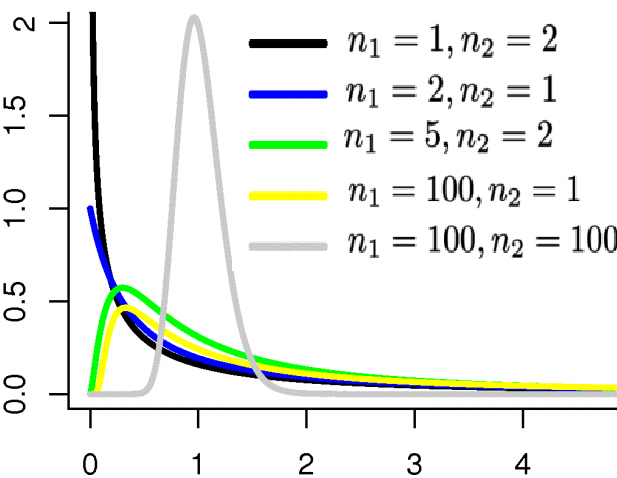
\includegraphics[width=4cm]{img/f.png}
		
		\textbf{PART 2}
		
		simple random sample : iid (independant and identically distributed) r.v.
		
		parameter : $\theta \equiv \theta(f) \in \Theta \subset \mathbb{R}^p$ (mean, median, variance)
		
		statistic : $h(X_1, ..., X_n)$
		
		$X\sim Be(p) \Rightarrow \hat{p}_n = \frac{1}{n}\sum^n X_i$
		
		sampling distribution : distr. of a statistic
		
		estimator of $\theta = \hat{\theta}_n = h(X_1,...,X_n)\in \Theta$
		
		$\hat{\mu}_n^{(k)} = \frac{1}{n}\sum^n X_i^k$
		
		$\hat{\sigma}_n^2 \equiv S_n^2 = \frac{1}{n-1}\sum^n(X_i - \overline{X})^2$
		
		$\hat{M}_n = X_{[(n+1)/2]}$ if n odd, $=(X_{[n/2]}+X_{[n/2+1]})/2$ else
		
		$\mathbb{E}(\overline{X}) = \mu\ \&\ \mathbb{V}ar(\overline{X})=\frac{\sigma^2}{n}$
		
		$\mathbb{E}(S^2) = \sigma^2\ \&\ \mathbb{V}ar(S^2)=\frac{1}{n}\left(\mathbb{E}((X_i-\mu)^4)-\frac{n-3}{n-1}\sigma^4\right)$
		
		$X\sim N(\mu,\sigma^2) \Rightarrow$
		
		1) $\frac{\overline{X}-\mu}{\sigma/\sqrt{n}}\sim N(0,1)$
		
		2) $\overline{X} \independent S^2$
		
		3) $(n-1)S^2/\sigma^2 \sim \chi_{n-1}^2$
		
		4) $\frac{\overline{X}-\mu}{S/\sqrt{n}}\sim t_{n-1}$
		
		5) $\sum X_i \sim N(n\mu,n\sigma^2)$
		
		$\forall \epsilon>0\ lim_{n\to \infty} P(|\overline{X}_n-\mu|>\epsilon)=0 : \overline{X}_n\overset{p}\to\mu$
		
		\textbf{Central limit theorem (CLT)}
		
		$X_i\ tq\ \mathbb{E}(X_i)=\mu\ \&\ \mathbb{V}ar(X_i)=\sigma^2 \Rightarrow \sum^n X_i \overset{n\to\infty}\approx N(n\mu,n\sigma^2)$
		
		$\Rightarrow Bin(n,p) \overset{n\to\infty}\approx N(np,npq)$ ($n>9\frac{max(p,q)}{min(p,q)}$) (continuity correction : $P(Bin\leq a) \approx P(N \leq a+0.5)$)
		
		$\Rightarrow Po(\lambda) \overset{\lambda\to\infty}\approx N(\lambda,\lambda)$
		
		$\Rightarrow Gamma(\alpha,\beta)\overset{\alpha\to\infty}\approx N(\alpha\beta,\alpha\beta^2)$
		
		$\Rightarrow \chi_n^2 \overset{n\to\infty}\approx N(n,2n)$
		
		\textbf{Point estimators}
		
		\textbf{unbiased} if $\mathbb{E}(\hat{\theta})=\theta$
		
		$\textbf{Bias}(\hat{\theta}) = \mathbb{E}(\hat{\theta})-\theta$
		
		Mean squared error : $\textbf{MSE}(\hat{\theta}) = \mathbb{E}\left[(\hat{\theta}-\theta)^2\right] = Bias^2(\hat{\theta}) + \mathbb{V}ar(\hat{\theta})$
		
		most efficient estimator : unbiased with smallest variance.
		
		$X_i \sim N(\mu,\sigma^2)$, $\mu$ known. $\widehat{\sigma^2} = \frac{1}{n}\sum^n(X_i-\mu)^2$ unbiased, but $\hat{\sigma} = \sqrt{\widehat{\sigma^2}}$ biased but asymptotically unbiased. $\hat{\sigma} = \sqrt{\pi/2}\frac{1}{n}\sum^n|X_i-\mu|$ unbiased.
		
		\textbf{consistent} if $P(|\hat{\theta}-\theta| > \epsilon) \overset{n\to\infty}\to 0$
		
		$MSE(\hat{\theta})\to 0 \Rightarrow \hat{\theta}$ consistent
		
		$\hat{\theta}$ consistent $\Rightarrow g(\hat{\theta})$ consistent (g continuous)
		
		\textbf{Method of Moments}
		
		$\hat{\mu}_k = \frac{1}{n}\sum^n X_i^k$
		
		solving $\hat{\mu}_k = \mu_k(\theta)$
		
		$\widehat{Var(X)} = \frac{1}{n}\sum(X_i-\overline{X}_n)^2$
		
		$Y_i \sim LN(\mu,\sigma^2) \Rightarrow$
		
		$\hat{\mu} = 2\ln\left(\frac{1}{n}\sum Y_i\right) - \frac{1}{2}\ln\left(\frac{1}{n}\sum Y_i^2\right)$
		
		$\hat{\sigma}^2 =  \ln\left(\frac{1}{n}\sum Y_i^2\right) - 2\ln\left(\frac{1}{n}\sum Y_i\right)$
		
		\textbf{Maximum Likelihood estimator (MLE)}
		
		joint PMF of observed sample : $L_n(\theta) = P(X_1=x_1,...,X_n=x_n|\theta) = f_n(x_1,...,x_n ; \theta) = \prod^n f(x_i ; \theta)$
		
		take the maximum of $L_n$.
		
		Via $\ln(L_n) = LL_n(\theta) = \sum \ln(f(x_i;\theta))$
		
		(derivate, anulate, check $2^{nd}$ derivate)
		
		Score function : $S_n(\theta) = (\frac{\partial LL}{\partial\theta_1}(\theta), \frac{\partial LL}{\partial\theta_2}(\theta))^T = 0$
		
		MLE is equivariant : $\hat{\theta}$ MLE of $\theta$ then $g(\hat{\theta})$ MLE of $g(\theta)$.
		
		$\hat{\theta}$ is consistent.
		
		$\hat{\theta}$ is \textbf{asymptotically normal} : $\hat{\theta}\approx N(\theta, I_n^{-1}(\theta))$ with
		
		$I_n(\theta) = -\mathbb{E}(H_{LL}(\theta)).$
		
		$H_{LL}(\theta) = \left( ^{\frac{\partial^2LL}{\partial\theta_1^2}}_{\frac{\partial^2LL}{\partial\theta_1\partial\theta_2}}\  _{\frac{\partial^2LL}{\partial\theta_2^2}}^{\frac{\partial^2LL}{\partial\theta_1\partial\theta_2}}\right)$
		
		\textbf{Cramer-Rao Lower Bound} : $I_n^{-1}(\theta)$
		
		$\hat{\theta}$ unbiased $\Rightarrow \mathbb{V}ar(\hat{\theta})\geq I_n^{-1}(\theta)$
		
		$g(\hat{\theta}) \approx N(g(\theta),(g'(\theta))^2 I_n^{-1}(\theta))$
		
		$X\sim Po(\lambda) \Rightarrow I_n(\lambda) = -\mathbb{E}(LL"(\lambda)) = \frac{n}{\lambda} \Rightarrow \hat{\lambda} = n^{-1}\sum X_i \approx N(\lambda,\lambda/n)$
		
		$\Rightarrow \hat{\theta} = n/\sum X_i \approx N(\theta,\frac{\theta^3}{n})$
		
		$X\sim Be(p) \Rightarrow I_n(p) = -\mathbb{E}(LL"(p)) = \frac{n}{pq} \Rightarrow \hat{p} = n^{-1}\sum X_i \approx N(p,pq/n)$
		
		$\Rightarrow \hat{\theta} = \ln(\hat{p}/(1-\hat{p})) \approx N(\theta,\frac{1}{npq})$
		
		\textbf{Confidence interval}
		
		two-sided with confidence level $(1-\alpha)100\%$ : $P(\hat{\theta}_L \leq \theta \leq \hat{\theta}_U) = 1-\alpha \Rightarrow [\hat{\theta}_L,\hat{\theta}_U]$ ($\alpha\in (0,1)$)
		
		$X\sim N : P(\overline{X}-z_{\alpha/2}\frac{\sigma}{\sqrt{n}}\leq \mu \leq \overline{X}+z_{\alpha/2}\frac{\sigma}{\sqrt{n}}) = 1-\alpha$
		
		lower one-sided : $P(\mu \geq \hat{\theta}_L) = 1-\alpha$
		
		Suppose we have a \textbf{pivotal statistic} ($Z(X,\theta)$ doesn't depends on $\theta$), search $P(a\leq Z(X,\theta)\leq b) = 1-\alpha$ and isolate $\theta$.
		
		ex : $X\sim N(\mu,\sigma^2) \Rightarrow \sqrt{n}\frac{\overline{X}-\mu}{S_n}\sim t_{n-1}$
		
		$(\independent X_i) \sim N(\mu_i,\sigma^2) \Rightarrow \frac{(\overline{X}_1-\overline{X}_2)-(\mu_1-\mu_2)}{\sigma\sqrt{1/n_1+1/n_2}}\sim N(0,1)$
		
		$\Rightarrow \frac{(\overline{X}_1-\overline{X}_2)-(\mu_1-\mu_2)}{S_p\sqrt{1/n_1+1/n_2}}\sim t_{n_1+n_2-2}$
		
		$S_p^2 = \frac{(n_1-1)S_1^2+(n_2-1)S_2^2}{n_1+n_2-2}$
		
		[L,U] for $\theta$ and g strictly monotonic $\Rightarrow$ $[g(L),g(U)] \cup [g(U),g(L)]$  for g($\theta$)
		
		asymptotically valid CI using $\hat{\theta} \approx N(\theta,\sigma^2)$ ($\sigma$ known or consistently estimated) (cfr CLT)
		
		\textbf{Hypothesis Testing}
		
		$H_0 : \theta \in \Theta_0\ vs\ H_1 : \theta\in\Theta_1$ with $\Theta_0\cup\Theta_1 = \Theta \ \&\ \Theta_0\cap\Theta_1 = \emptyset$
		
		$H_0$ : null hypothesis vs $H_1$ : alternative hypothesis.
		
		test statistic (regarding statistic $T_n(X)$)
		
		$R \subset Range(T)$ leading to reject $H_0$ : rejection region or critical region.
		
		$P(Type\ I\ error) = \alpha = P(RH_0|H_0)$ : significant level of the test
		
		$P(Type\ II\ error) = \beta = P(AH_0|H_1)$
		
		State hypothesis, fix $\alpha$, chose $R_{\alpha,n}$ tq $P(T(X)\in R|H_0) = \alpha$, calculate $T(x)$, conclude (reject or don't know (accept if $\beta$ small))
		
		\textbf{P-Value}
		
		$T_n(X)$ a test statistic such that small T $\Rightarrow$ false $H_0$.
		
		$p_n(x) = P(T_n(X) \leq T_n(x)|H_0)$
		
		p-value is the probability to be at least this extreme given $H_0$. More informative than a critical value (nuances).
		
		if $\sigma_1^2 = \sigma_2^2$ : $F = \frac{S_1^2}{S_2^2}\sim F_{n_1-1,n_2-1}$
		
		We can use asymptotically valid tests under conditions.
		
		\textbf{Integral reminders}
		
		Fubini : $\iint_A f(x,y)dxdy = \int_{y_{min}}^{y_{max}}\left(\int_{A_y}f(x,y)dx\right)dy$ ($A_y = \{x : (x,y)\in A\}$)
		
		Leibniz : $\frac{d}{dy}\left(\int_{a(y)}^{b(y)}f(x,y)dx\right) = \int_{a(y)}^{b(y)}\frac{\partial f}{\partial y}(x,y)dx + f(b(y),y)b'(y) - f(a(y),y)a'(y)$
		
		Chain Rule : $(x,y)\to z(s(x,y),t(x,y))\in\mathbb{R}$
		
		$\frac{\partial z}{\partial x}(a,b) =$
		
		$\frac{\partial s}{\partial x}(a,b)\frac{\partial z}{\partial s}(s(a,b),t(a,b))$
		
		$+ \frac{\partial t}{\partial x}(a,b)\frac{\partial z}{\partial t}(s(a,b),t(a,b))$
		
	\end{multicols}
	
	
	
\end{document}
